%!TEX root=report.tex
\section{Data}

The GRACE dataset can be downloaded from GRGS \cite{GRACE-data-source}.
In this analysis it is the EWH dataset from release 2 in the GRGS format with a 10-day interval.

This dataset contains a quite a few text files, each contain information in its filename and its content.
The filenames have the format:

\begin{lstlisting}
grid.water.10day_model_minus_RL02MF.19202_19211.txt
grid.water.10day_model_minus_RL02MF.19212_19221.txt
...
\end{lstlisting}

In the filename, it is the last two numbers (e.q. \texttt{19202\_19211}) there are important.
These numbers contains the start and end date for the file content.
Both numbers are the amount of days since ``1950-01-01'', where the first number is the start date and the last number is the end date. \cite{GRACE-data-format-dates}

The actual content of each text file should be read as a ``Space Separated Values'' format.
When this is done one will have a $6480 \times 10$ matrix, this should then be \texttt{reshape}'ed row-wise intro a $180 \times 360$ matrix.
The result are a matrix with decreasing latitude on the rows and increasing longitude on the columns. \cite{GRACE-data-format-grids}

\subsection{Data example}

\begin{figure}[H]
	\centering
	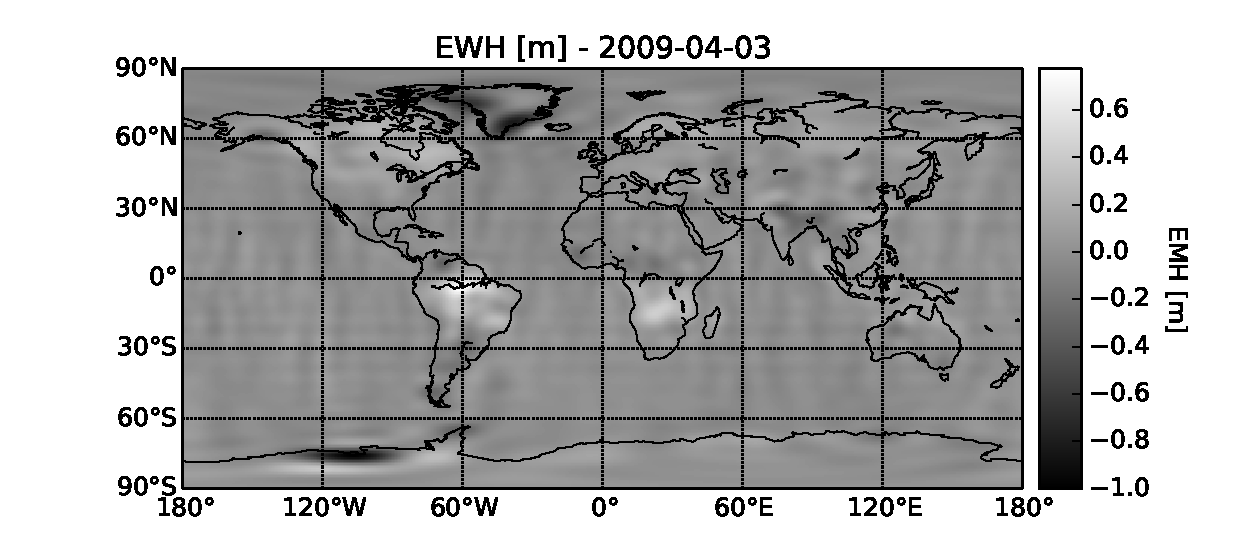
\includegraphics[width=\textwidth]{figures/data-example-world}
	\caption{Plot of the data from 3 April 2009}
	\label{fig:data-example-world}
\end{figure}

\begin{figure}[H]
	\centering
	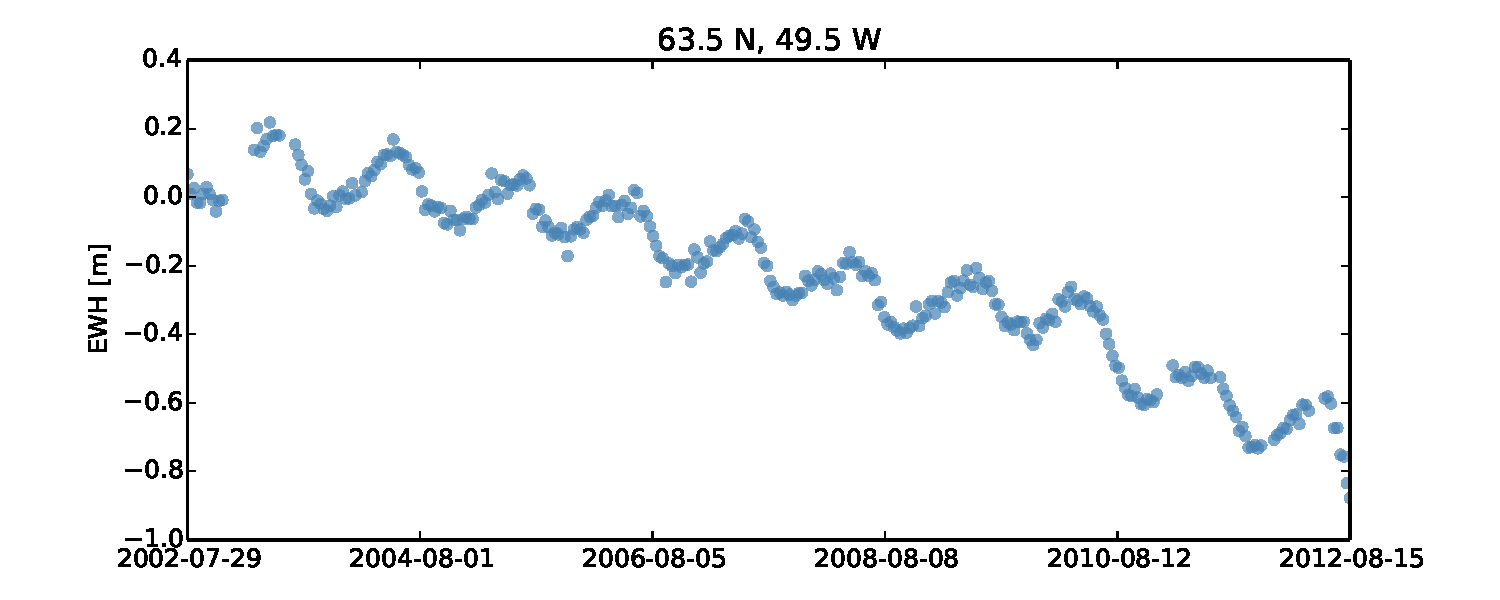
\includegraphics[width=\textwidth]{figures/data-example-scatter}
	\caption{Plot of EWH at 63.5 N 49.5 W, west coast of Greenland.}
	\label{fig:data-example-scatter}
\end{figure}

From Figure \ref{fig:data-example-world} a local mass loss at Greenland and the South Pole is seen, this is likely caused by the ice melting.
A mass increment at South America can also been seen, this is likely caused by the rainy season.
On Figure \ref{fig:data-example-scatter}, mass loss with a yearly periodic trend is seen.
